\section{Wstęp}
\label{sec:wstep}
Celem pracy było zbadanie możliwośći integracji modułów \texttt{ESP8266} z koncepcją  Internetu Rzeczy (ang. Internet of Things, IoT). Cel osiągnięto poprzez stworzenie infrastruktury na którą składają się urządzenia ESP8266 ze szczególnym uwzględnieniem \texttt{topologii}, \texttt{niezawodności} jak i \texttt{uniwersalności} systemu. W pracy zbudowany został rozproszony system bazujący na układach ESP8266, realizujący komunikację z \texttt{mobilnym serwerem}.

Zaimplementowano dwa rozwiązania tego problemu, jedno bazujące na działającym, na każdym urządzeniu serwisie \texttt{telnet}, natomiast drugie na web serwisie \texttt{CoAP}. Zweryfikowana została hipoteza o możliwości integracji modułów ESP8266 z koncepcją internetu rzeczy i możliwością dynamicznego rozszerzenia stworzonego systemu.

\subsection{Motywacja - charakterystyka problemu}
Istotą Internetu rzeczy (ang. Internet of Things, IoT) jest możliwość połączenia w sieć każdego rodzaju urządzeń. Koncepcja ta zakłada stworzenie takiej infrastruktury, która połączy ze sobą urządzenia codziennego użytku, w calu dostarczenia nowych funkcjonalności i usług. W nadchodzącym czasie będziemy mieli możliwość obserwacji jak fundamentalnie zmienia się możliwość integracji świata fizycznego, ze światem urządzeń cyfrowych. 

Współcześnie istnieje bardzo wiele urządzeń komunikujących się ze sobą, tworzących swoistą sieć, nazwaną Internet rzeczy\cite{iot-art}. Jest to koncepcja, wedle której jednoznacznie identyfikowalne przedmioty mogą pośrednio lub bezpośrednio gromadzić, przetwarzać lub wymieniać dane za pośrednictwem sieci komputerowej. 

Na rynku istnieje kilka rozwiązań pozwalających na zarządzanie tymi urządzeniami. Są to między innymi opisane szerzej w \autoref{sec:existing-systems} Contiki OS, Windows 10 IoT Core, Raspberry Pi czy Zetta. Celem pracy było stworzenie systemu o podobnej funkcjonalności, pozwalającej użytkownikom zarządzać, zbierać dane, sterować różnymi urządzeniami. Użytkownicy mają mieć wygodny i prosty w obsłudze interfejs. 

Przyczyna powstania pomysłu, oraz problem i cel projektu, mając na uwadze przedstawione powyżej \texttt{tezy}, można formalnie przedstawić następująco:

\begin{itemize}
	\item \texttt{Przyczyna:} Diametralnie zwiększająca się ilość urządzeń wchodzących w skład Internetu rzeczy\cite{iot-art}.
	\item \texttt{Problem:} Stworzenie uniwersalnego interfejsu do efektywnego zarządzania tymi urządzeniami.
	\item \texttt{Rozwiązanie:} Dostarczenie modelu działającego w uproszczonym środowisku, dostarczającego wysokopoziomowy interfejs.
\end{itemize}

\subsection{Przegląd istniejących rozwiązań}
\label{sec:existing-systems}
Możliwość zdalnego konfigurowania urządzeń wchodzących w skład Internetu rzeczy przez użytkownika końcowego, bądź też samodzielnego działania układu w koncepcji IoT posiada niezliczoną ilość zastosowań w wielu obszarach, takich jak:

 \begin{itemize}
	\item Mieszkania,
	\item Miasta,
	\item Przemysł,
	\item Transport
\end{itemize}

Istnieje kilka projektów adresujących ten problem. Przykładowe z nich to Contiki OS, Windows 10 IoT Core, Raspberry Pi oraz Zetta. Zapoznanie się z nimi, z rozwiązaniami w nich stosowanymi oraz z oferowanymi przez nie interfejsami pozwoliło uniknąć wielu błędów i problemów występujących podczas projektowania własnego systemu.

\paragraph{Contiki OS}\cite{contiki-www} (The Open Source OS for the Internet of Things) \texttt{Contiki} łączy małe, tanie i energooszczędne mikrokontrolery z internetem. Contiki wspiera w pełni standard \texttt{IPv6} i \texttt{IPv4}, wraz z energooszczędnymi bezprzewodowymi standardami: \texttt{6lowpan}, \texttt{RPL}, \texttt{CoAP}. 

Contiki oferuje łatwe i szybkie tworzenie oprogramowania, aplikacje są pisane w czystym C, wraz z symulatoram \texttt{Cooja} systemy te mogą być emulowane przed wrzucemeniem ich na hardware. Środowisko jest dostępne i całkowicie darmowe, co jest dużym plusem oprogramowania Contiki.

Contiki można uruchomić na wielu energooszczędnych, bezprzewodowych urządzeniach, takich jak\cite{contiki-hardware-www}: \texttt{CC2538}, \texttt{Sensortag}, \texttt{CC2650}

\paragraph{Windows 10 IoT Core}\cite{windows-iot-www} to również system operacyjny, jest to wersja Windows 10, która została zoptymalizowana dla małych urządzeń bez wyświetlacza, oraz które są uruchamiane na \texttt{Raspberry Pi} 2 i 3, \texttt{Arrow DragonBoard 410c} i \texttt{MinnowBoard MAX}. 
Windows 10 IoT Core wykorzystuje bogate, uniwersalne \texttt{API - Universal Windows Platform (UWP)}. UWP API pozwala na tworzenie aplikacji, która może być używana na wielu urządzeniach, telefonach lub komputerach i udostępnia dostęp do tysięcy urządzeń Windows, które można wykorzystywać w projekcie.

Windows 10 IoT Core wspiera łatwe w użyciu Arduino Wiring API używane w Arduino, oraz biblioteki do pezpośredniego dostępu do urządzeń. Aby tworzyć aplikacje można również używać narzędzia Visual Studio.


\paragraph{Raspberry Pi}\cite{raspberry-www} w odróżnieniu od prezentowanych tutaj rozwiązań jest to platforma komputerowa, która może posiadać zainstalowany system Linux, jak i Windows 10 IoT Core.

\paragraph{Zetta}\cite{zetta-www} (An API-First Internet of Things Platform) jest to platforma open source zbudowana na Node.js, aby zapewnić możliwość tworzenia serwerów Internetu Rzeczy, które są uruchomione na rozproszonych komputerach. Zetta łączy REST API, WebSockets i reaktywne programowanie - idealne dla łączenia wielu urządzeń w data-intensive, aplikacje czasu rzeczywistego.

\paragraph{Podsumowanie:} Pomijając aspekty techniczne, przedstawione systemy mają kilka ważnych, łatwo widocznych cech wspólnych, które powinien posiadać również system implementowany w ramach projektu:

\begin{itemize}
	\item efektywna komunikacja np. standard Wi-Fi
	\item energooszczędność urządzeń, mimo ciągłej aktywności
	\item responsywność oraz stabilnosć systemu
	\item niezawodność komunikacji
\end{itemize}


\section{Sformułowanie problemu}
\label{sec:sformulowanie-problemu}
Zawiera precyzyjne, wyczerpujące sformułowania problemów badawczego i projektowego, jakie zostaną w pracy rozwiązane. Są one odniesione do aktualnego stanu wiedzy, co potwierdzać muszą stosowne referencje. Ta część pracy zawiera w szczególności analizę zapotrzebowań projektu software będącego pożądanym składnikiem pracy magisterskiej w naukach technicznych w dyscyplinie informatyka.

\subsection{Problem badawczy - struktura IoT}
Internet Rzeczy należy rozumieć jako system, w którym przedmioty mogą komunikować się między sobą, za pośrednictwem człowieka lub bez jego udziału.
Dobrym schematem obrazującym tą koncepcję jest \autoref{fig:iot_base}. Widać tutaj wyraźnie, że to podejście jest uniwersalne. Z rysunku wynika, że istnieje podział na cztery główne części:

\begin{figure}[!htbp]
	\centering
	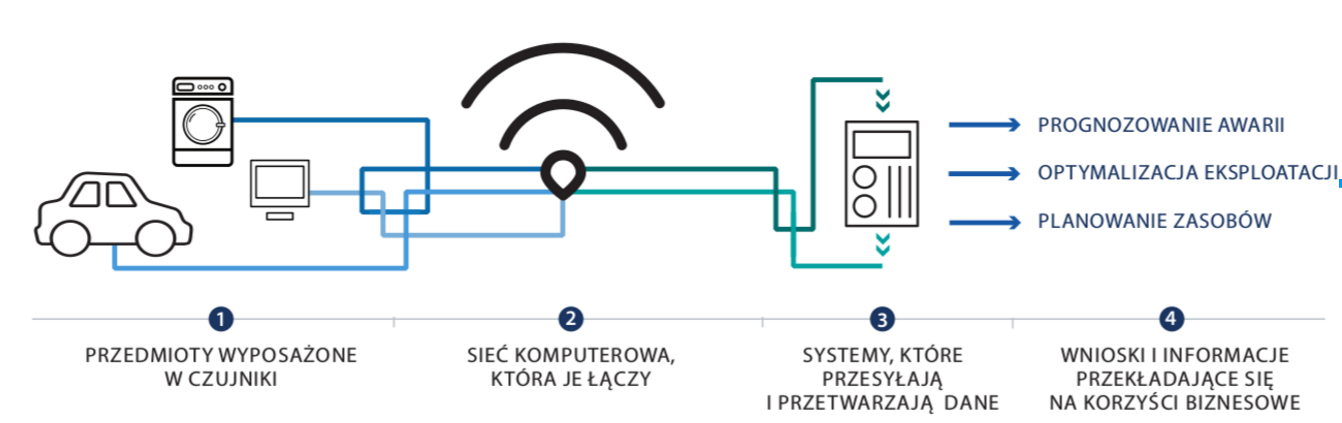
\includegraphics[width=1.0\textwidth]{images/iot.png}
	\caption[Idea funkcjonowania rozwiązań Internetu Rzeczy.]{Idea funkcjonowania rozwiązań Internetu Rzeczy}
	\label{fig:iot_base}
\end{figure}

\subsubsection{Przedmioty wyposażone w czujniki}
Naszą sieć IoT możemy zbudować praktycznie w każdej dziedzinie. ża pomocą jednego systemu mamy możliwość sterowania każdym rodzajem urządzeń - od sprzętów AGD/RTV po samochody, czy domy. Sfery zastosowań urządzeń IoT przedstawia \autoref{fig:zastosowania_iot}. Widać wyraźnie, że istnieją one wszędzie, potwierdzeniem tego faktu jest \autoref{fig:ile_urzadzen} opisany szerzej w \autoref{sec:benefits_conclusions}.

\begin{figure}[!htbp]
	\centering
	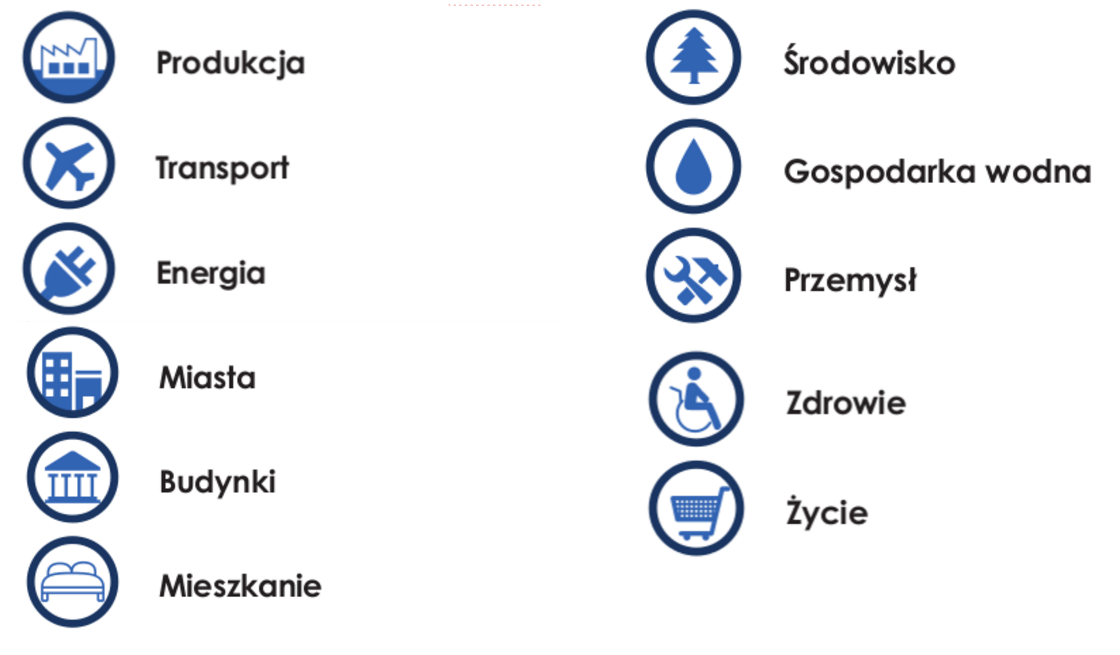
\includegraphics[width=1.0\textwidth]{images/zastosowania.png}
	\caption[Obszar zastosowania IoT.]{Obszar zastosowania IoT}
	\label{fig:zastosowania_iot}
\end{figure}
\subsubsection{Sieć komputerowa, która je łączy}
Tutaj mamy pole do popisu, bo tak naprawdę istnieje bardzo wiele interfejsów pozwalających na łączenie urządzeń w jedną integralną całość. Do wyboru mamy od tych bardziej znanych standardów m.in:

\begin{itemize}
	\item Wi-Fi
	\item Bluetooth
\end{itemize}
Po te mniej znane, jednak równie często wykorzystywane:
\begin{itemize}
	\item NFC 
	\item Z-Wave 
\end{itemize}

\subsubsection{Systemy, które przetwarzają i przesyłają dane}
Posiadając już podpięte urządzenia do sieci, musimy jeszcze mieć czym nimi sterować/przetwarzać dane itp. Mamy możliwość instalacji urządzeń tych bardziej profesjonalnych, dedykowanych dla konkretnego klienta, jak np. \autoref{fig:panel_ogrzewanie}. Jest to panel do sterowania ogrzewaniem w domu firmy proav. Poprzez te bardziej uniwersalne, jak chociażby smartphone z systemem android/ios/windows.

\begin{figure}[!htbp]
	\centering
	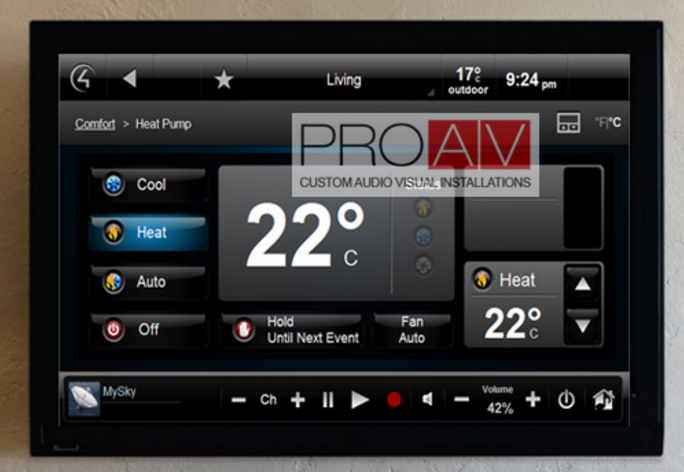
\includegraphics[width=1.0\textwidth]{images/panel_ogrzewanie.png}
	\caption[Panel do sterowania ogrzewaniem.]{Panel do sterowania ogrzewaniem}
	\label{fig:panel_ogrzewanie}
\end{figure}

\subsubsection{Wnioski i informacje przekładające się na korzyści biznesowe}
\label{sec:benefits_conclusions}
Innym zobrazowaniem idei Internetu Rzeczy jest \autoref{fig:iot_short}. Widać tutaj wszystko to co zostało po krótce przedstawione w tym rozdziale. 
Ważnym wyznacznikiem, który przekonał mnie do napisania tej pracy był fakt, że libczba urządzeń IoT drastycznie wzrasta w czasie. Przedstawia to \autoref{fig:ile_urzadzen}, przewidywania są takie, że ich liczba do 2020 wzrośnie do 25 bilionów i już dawno przekroczyła liczbę ludności na świecie.  
\begin{figure}[!htbp]
	\centering
	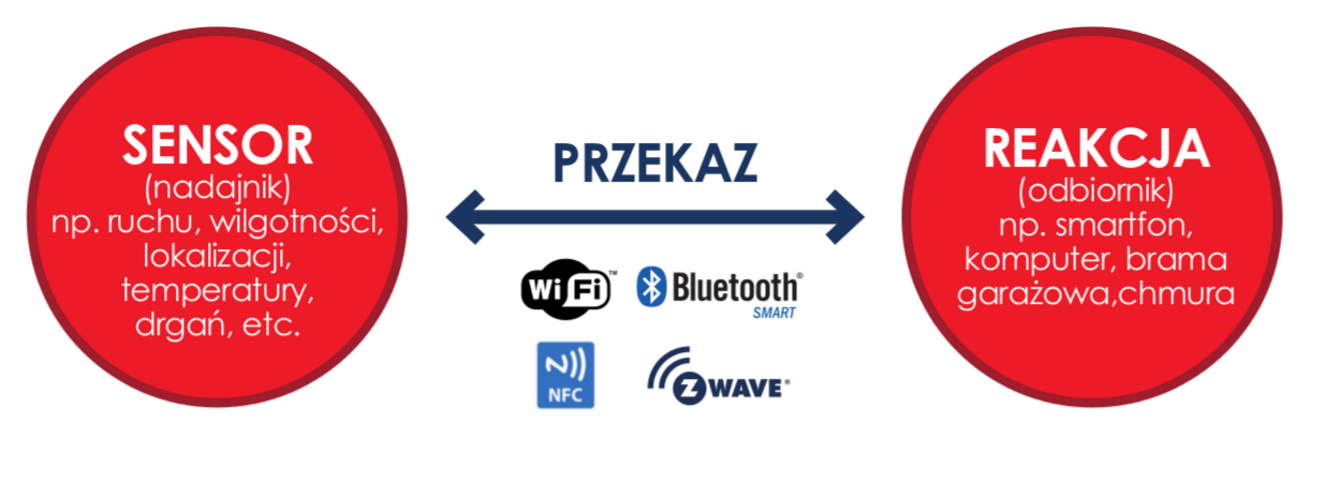
\includegraphics[width=1.0\textwidth]{images/iot_short.png}
	\caption[System wymiany informacji.]{System wymiany informacji}
	\label{fig:iot_short}
\end{figure}
\begin{figure}[!htbp]
	\centering
	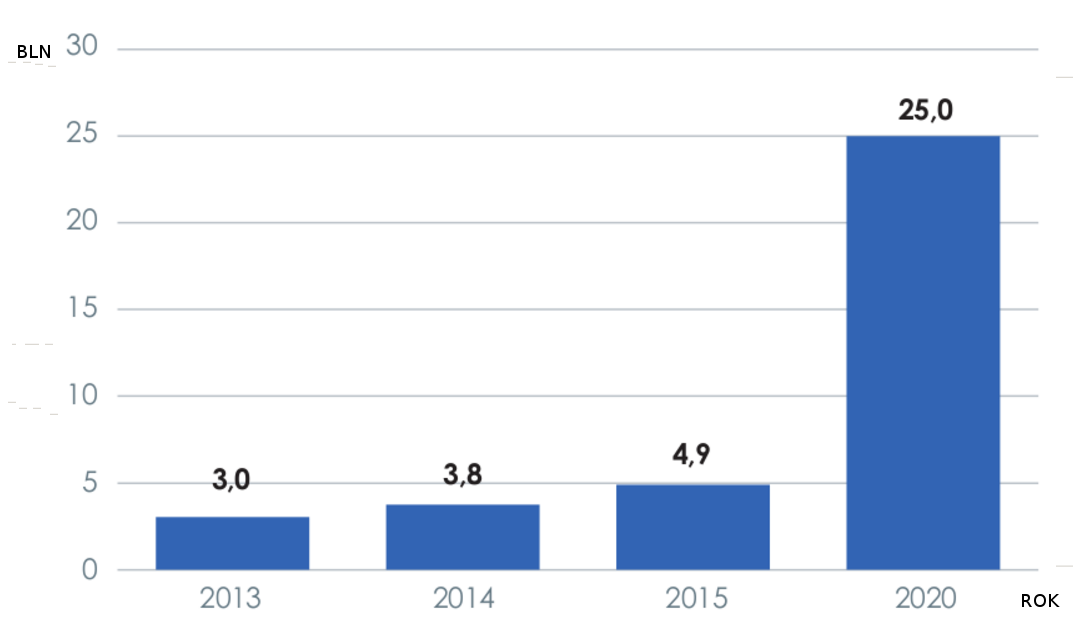
\includegraphics[width=1.0\textwidth]{images/ile_urzadzen.png}
	\caption[Liczba urządzeń Internetu Rzeczy.]{Liczba urządzeń Internetu Rzeczy}
	\label{fig:ile_urzadzen}
\end{figure}


\subsection{Problem projektowy}

\subsection{Analiza zagrożeń}
Wykonalność projektu jest obarczona pewnym ryzykiem. Jest ono głównie związane z możliwą nieznajomością obranych w późniejszym czasie technologii oraz małym dościadczeniem w dziedzinie Internetu rzeczy.

Kolejnym zagrożeniem jest ograniczony czas. Proponowane rozwiązanie zakłada stworzenie prototypu urządzenia, a następnie aplikacji, więc swtorzenie układu będzie konieczne do uruchomienia i przetestowania całości.


\section{Metodyka rozwiązania}
\label{sec:metodyka-rozwiazania}
W tej części opisane są szczegółowo metody rozwiązania postawionego problemu. Opis ten powinien być precyzyjny, wyczerpujący i zgodny z aktualnym formalizmem oraz terminologią specyficznymi dla dziedziny pracy. Powinien on w szczególności zawierać definicje stosowanych metod numerycznych, algorytmów oraz struktur danych.

\subsection{Rozwiązanie bazujące na standardzie telnet}
Finalnym produktem powinien być stabilny prototyp urządzenia, połączony z modułem ESP8266, posiadający przynajmniej jeden czujnik. Użytkownik powinien mieć możliwość zdalnego starowania tym urządzeniem za pomocą mobilnej aplikacji. System powinien składać się przynajmniej z trzech urządzeń, każde z nich powinno aputomatucznie łączyć się do sieci Wi-Fi po uruchomieniu. 

Dodatkowo, system powinien oferować wygodny interfejs dostępny dla użytkownika końcowego. Udostępnienie API poprzez sterowanie urządzeniami za pomocą telnetu pozwoli na programowy dostęp do sterowania urządzeń z poziomu dowolnego języka programowania. Powinny również zostać zaimplementowane mechanizmy autentykacji zlecanych operacji. Oprócz dostępu programowego, planowana jest implementacja graficznego interfejsu mobilnego, przeznaczonego dla użytkowników\cite{kukdm-art}.

\begin{figure}[!htbp]
	\centering
	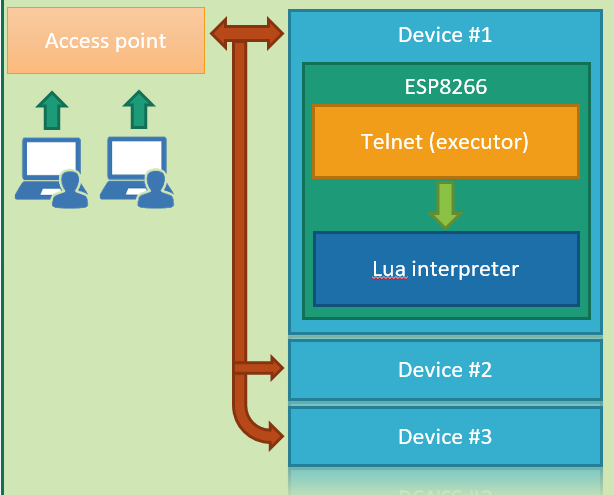
\includegraphics[width=0.9\textwidth]{images/fig01-arch-overview.png}
	\caption[Wizja architektury systemu.]{Wizja miejsca użytkownika, budowy urządzenia, oraz sposobu komunikacji}
	\label{fig:arch-overview}
\end{figure}

Wizję budowy urządzenia przedstawia \autoref{fig:arch-overview}.

\subsection{Rozwiązanie bazujące na CoAP Web Service}

\begin{figure}[!htbp]
	\centering
	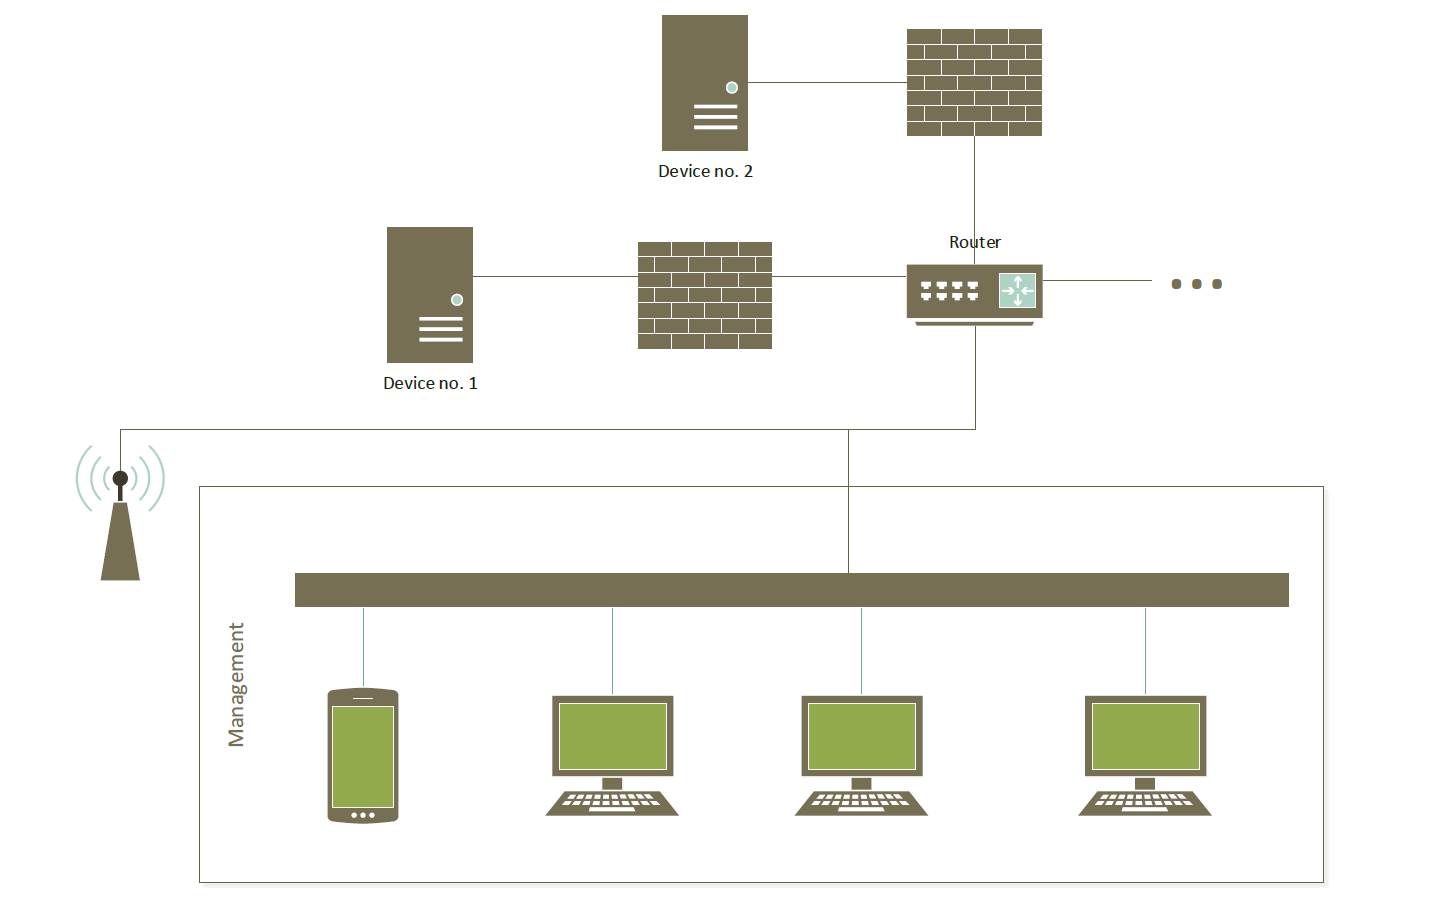
\includegraphics[width=0.9\textwidth]{images/schemat.png}
	\caption[Wizja architektury systemu w standardzie CoAP.]{Wizja miejsca użytkownika, sposobu komunikacji w systemie w standardzie CoAP}
	\label{fig:schemat}
\end{figure}
Wizję budowy urządzenia przedstawia \autoref{fig:schemat}.

\section{Podsumowanie i wnioski}
\label{sec:podsumowanie-wnioski}
Podsumowanie stanowi krótkie streszczenie zawartości pracy uwypuklające oryginalne wyniki autora. Zawiera ono również krótkie uzasadnienie dla weryfikacji tezy pracy, oparte na tych wynikach. Wnioski powinny dotyczyć stopnia realizacji przyjętego plany badawczo – projektowego oraz możliwości jego kontynuacji, jak również możliwości zastosowania uzyskanych i planowanych rezultatów w praktyce.


